\documentclass{article}

\usepackage{graphicx} % for images
\usepackage{amsmath} % for math
\usepackage{amssymb} % for \mathbb
\usepackage{siunitx} % for \SI, \num
\usepackage{hyperref} % for \url{}

% This stuff is for figures
\usepackage{float}
\DeclareGraphicsExtensions{.pdf, .png, .jpg}

% coloring of links for PDF format
\hypersetup{
    colorlinks=true,
    urlcolor=blue,
    linkcolor=black
}

% \c command redefinition (for monospaced font)
\renewcommand{\c}[1]{\texttt{#1}}
% \today command re-definition
%https://tex.stackexchange.com/questions/112932/today-month-as-text
\renewcommand{\today}{\ifnum\number\day<10 0\fi \number\day \space%
\ifcase \month \or January\or February\or March\or April\or May%
\or June\or July\or August\or September\or October\or November\or December\fi\space%
\number \year} 

\begin{document}

\noindent
Rodrigo Becerril Ferreyra\\
CECS 361 Section 01\\
Lab 5\\
\today

%\addcontentsline{toc}{section}{Introduction}
\section{Introduction} The purpose of this laboratory assignment
was to practice knowledge of faults and fault checking.
Specifically, given a faulty module
(with a stuck-at-one fault)
and the diagram of the
circuit it was supposed to implement, the task was to find where
the fault was located via two methods: the first
is the activation--propagation method, and the second is
an equivalence method that was implemented on the Nexys A7
100T FPGA board.

The activation--propagation method consists of
finding all the possible places that a stuck-at-one fault could
be, either by using gate-oriented fault collapsing or
line-oriented fault collapsing. The next step is to activate
and propagate the faults. Lastly, if the line being tested
is stuck at one, then the activation of the fault will not
cause the desired result. The equivalence method, on the other
hand, is more simple:
the output produced by the faulty circuit
using each set of inputs is
tested against the expected output from a flawless circuit;
the faulty circuit's functionality is tested for equivalence
with a circuit that is known to work. This method was
implemented on the board: both circuit's inputs are driven
by on-board switches, and if any output from both circuits
doesn't match, a light flashes with the following color order:
red, green, blue.

For reference, the Figure \ref{diagram:original}
is the desired (non-faulty) circuit
that was implemented in this lab.

\begin{figure}[H]
    \centering
    \includegraphics[width=\textwidth]{Images/Circuit_diagram_clean}
    \caption{Desired, non-faulty circuit.}
    \label{diagram:original}
\end{figure}

\section{Activation--Propagation Method} As previously stated,
this method involves finding all the places where a
stuck-at-one fault can be, and testing them individually.
Figure \ref{diagram:faulty} is a diagram of all
possible stuck-at-X faults, obtained using the
line-oriented fault collapsing method. All of the different
places where a stuck-at-one fault can be found are labeled.
Note that the two stuck-at-zero faults are not labeled,
because we knew prior to testing that the fault was a
stuck-at-one fault.

\begin{figure}[H]
    \centering
    \includegraphics[width=\textwidth]{Images/Circuit_faults}
    \caption{Possible stuck-at-X locations.}
    \label{diagram:faulty}
\end{figure}

Activating the fault means giving the line it's on the opposite
value; to activate a stuck-at-one fault, the line being tested
for a fault must be set to zero using the correct combination
of inputs. Propagating the fault consists of choosing the
correct combination of inputs such that no gate on the fault's
path has a controlling value; in practice, this means making
sure that no AND gate has a zero and no OR gate has a one
on its input (an XOR gate does not have a controlling value).
To make it easier to see on a waveform, I also flipped the
value of the line being tested; if the line is truly
``stuck,'' then there will be no change in the output.

Figure \ref{waveform:faultdetection} below shows the result
of all twelve tests, while Table
\ref{table:activation-propagation} shows the values
used to test each case.

\begin{figure}[H]
    \centering
    \includegraphics[width=\textwidth]{Images/"fault detection"}
    \caption{Activation--propagation test results.}
    \label{waveform:faultdetection}
\end{figure}
\begin{table}[H]
    \centering
    \resizebox{\textwidth}{!}{%
\begin{tabular}{c||c|c|c|c|c|c|c|c|c|c|c|c}
Fault & S1 & S2 & S3 & S4 & S5 & S6 & S7 & S8 & S9 & S10 & S11 & S12 \\ \hline
\c{\{a, b, c\}} & 011 & 101 & 100 & 011 & 101 & 001 & 101 & 011 & 010 & 001 & 001 & 101
\end{tabular}%
}
    \caption{Test cases to activate and propogate a stuck-at-one fault.}
    \label{table:activation-propagation}
\end{table}

It may not be obvious from the waveform, but this test
shows that there is a stuck-at-one fault at S06, S10, and
S11. Flipping S06 was expected to change both outputs,
but F1 did not change. The same happened while testing S10
and S11, which is to be expected, as these lines are connected
to each other.

Since S06 does not connect to anything other than S10 and S11,
the possible combinations of faults are as follows: fault
at S06 only, fault at S10 and S11 only, or fault at S06, S10,
and S11. These three cases are indistinguishable.

\section{Equivalence Method} This method consists of testing
the faulty outputs with the expected ones. To do this,
I created the expected functionality of the circuit in
Figure \ref{diagram:original}, structurally, in
Verilog. The resulting circuit diagram can be seen in
Figure \ref{diagram:expected}.

\begin{figure}[H]
    \centering
    \includegraphics[height=\textwidth, angle=-90]{Images/"schematic expected"}
    \caption{Verilog schematic diagram of expected (non-faulty) circuit.}
    \label{diagram:expected}
\end{figure}

The respective \c{F0} and \c{F1} outputs of both (faulty and
non-faulty) modules were then XOR'd together, and the OR
of these XOR outputs activated the RGB LED flash mechanism.

\subsection{RGB LED Flash Mechanism} The flashing was
implemented using a Moore Finite State Machine model.
It takes two inputs and outputs three signals: its inputs
are \c{enable} and \c{tick}, and its outputs are \c{red\_on},
\c{green\_on}, and \c{blue\_on}. The \c{enable} input is
driven by the XOR/OR described above, and the \c{tick}
input is driven by a \SI{0.5}{s}, one-clock-wide pulse.
The outputs are meant to control the red, green, and blue
LEDs on the board, respectively. The
state transition diagram, table, and outputs are shown
in Figure \ref{fsm} below.

\begin{figure}[H]
    \centering
    \includegraphics[width=\textwidth]{Images/fsm}

    \begin{tabular}{|c|cccc|}
        \hline
        Input = \{enable, tick\} & \multicolumn{4}{c|}{Next state} \\ \cline{1-1}
        state & 0 & 1 & 2 & 3 \\ \hline
        off & off & off & off & red \\
        red & off & off & red & green \\
        green & off & off & green & blue \\
        blue & off & off & blue & red \\ \hline
    \end{tabular}

    \begin{tabular}{|c|c|}
        \hline
        State & Outputs = \{red, green, blue\} \\ \hline
        off & 000 \\
        red & 100 \\
        green & 010 \\
        blue & 001\\ \hline
    \end{tabular}
    \caption{FSM state transition diagram, table, and outputs (Moore).}
    \label{fsm}
\end{figure}

\subsection{Truth Table} Of course, this task can also be
achieved by using a truth table, and comparing the results
of the expected outputs to the faulty outputs.

\begin{table}[H]
    \centering
    \begin{tabular}{c|cc|cc}
        & \multicolumn{2}{c|}{Actual} & \multicolumn{2}{c}{Expected} \\
       \{a, b, c\} & \multicolumn{1}{c|}{F1} & F0 & \multicolumn{1}{c|}{F1} & F0 \\ \hline
       000 & 0 & 0 & 0 & 0 \\
       001 & \textbf{1} & 1 & \textbf{0} & 1 \\
       010 & 0 & 1 & 0 & 1 \\
       011 & 1 & 0 & 1 & 0 \\
       100 & 0 & 1 & 0 & 1 \\
       101 & 1 & 0 & 1 & 0 \\
       110 & 1 & 0 & 1 & 0 \\
       111 & 1 & 1 & 1 & 1
    \end{tabular}
    \caption{Expected and faulty outputs}
    \label{truthtable}
\end{table}

It is evident that in the input combination
\c{\{a, b, c\} = 3'b001}, the output value of F1 differs
between the actual (faulty) circuit and the expected circuit.
This is also where the hardware-implemented RGB LED flashes.

\subsection{Top-Level Diagram} Figure \ref{diagram:top-level}
displays the schematic diagram of the top-level module,
which is implemented on the board (feel free to zoom in).

From this diagram, it is clear how both circuits share
the same inputs, and how the differences in
corresponding outputs from both circuits are detected.
A two-input XOR gate's output is high whenever its inputs
are different, so if there is any difference between either
set of inputs (or both), the OR gate will go high and activate
the RGB flash mechanism.

\begin{figure}[H]
    \centering
    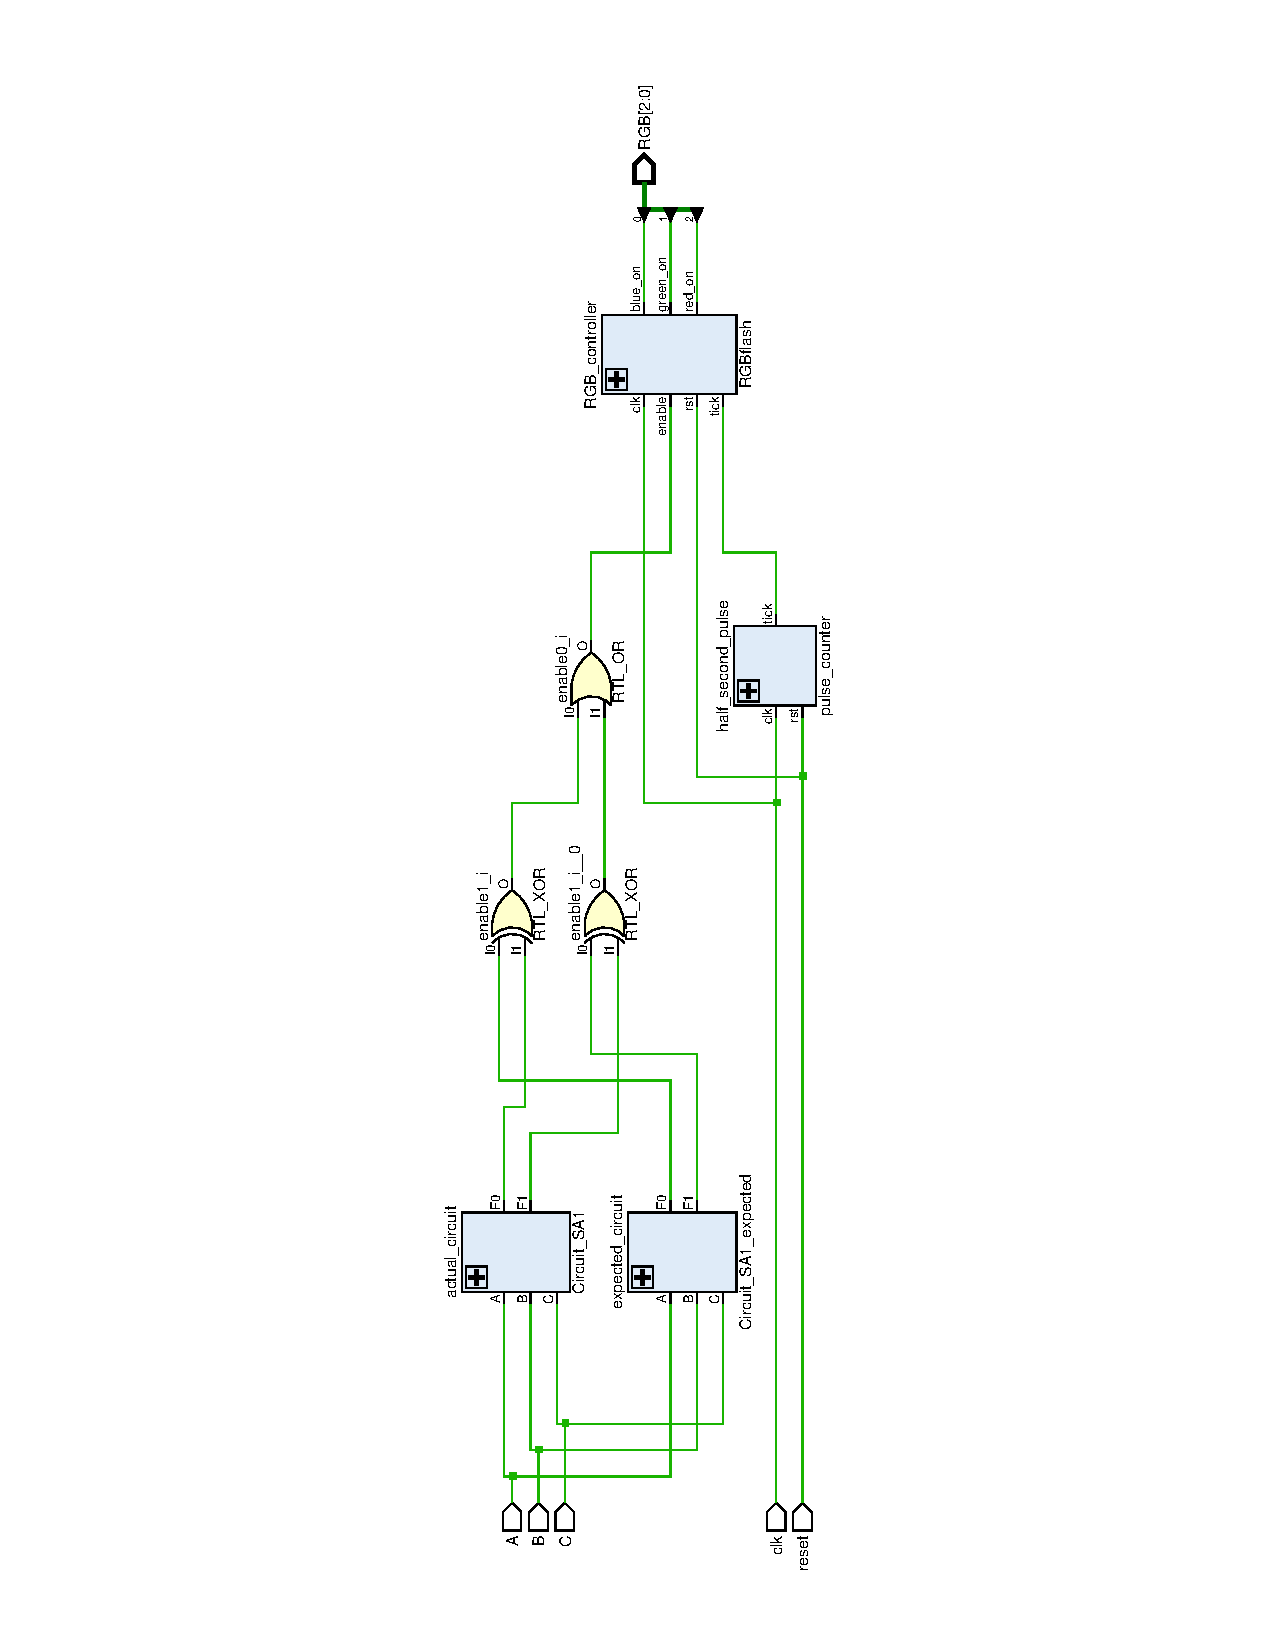
\includegraphics[height=\textwidth, angle=-90]{Images/schematic_toplevel}
    \caption{Top-level board implementation.}
    \label{diagram:top-level}
\end{figure}

\section{Waveforms and Testing} The truth table in
Table \ref{truthtable} was achieved by testing the given
circuit with all \(2^3 = 8\) permutations of inputs.
In addition, the expected circuit shown in Figure
\ref{diagram:expected} is also displayed for comparison.
Figure \ref{waveform:comparison} shows the combinations
of inputs and their respective outputs for both circuits.

\begin{figure}[H]
    \centering
    \includegraphics[width=\textwidth]{Images/"Circuit_SA1_waveform comparison"}
    \caption{Waveform for given (faulty) circuit.}
    \label{waveform:comparison}
\end{figure}

The differences between these two pairs of inputs can be seen
clearly when \(i = 1\) (or equivalently when
\c{\{a, b, c\} = 3'b001}).

Figure \ref{picture:board} shows the board implementation
when either of the outputs from both circuits don't match,
and when all corresponding outputs match.

\begin{figure}[H]
    \centering
    \includegraphics[height=0.49\textwidth, angle=-90]{Images/20201129_123140}
    \includegraphics[height=0.49\textwidth, angle=-90]{Images/20201129_123208}
    \caption{Mismatched and matching outputs on the board.}
    \label{picture:board}
\end{figure}

\end{document}

Simple truth table:
\begin{tabular}{l|llllllll}
    \{a, b, c\} & 000 & 001 & 010 & 011 & 100 & 101 & 110 & 111 \\ \hline
    F1 & 0 & 1 & 0 & 1 & 0 & 1 & 1 & 1 \\ \cline{1-1}
    F0 & 0 & 1 & 1 & 0 & 1 & 0 & 0 & 1
\end{tabular}

Extended (comparison) truth table:
\begin{tabular}{c|cc|cc}
    & \multicolumn{2}{c}{Actual} & \multicolumn{2}{c|}{Expected} \\
   \{a, b, c\} & \multicolumn{1}{c|}{F1} & F0 & \multicolumn{1}{c|}{F1} & F0 \\ \hline
   000 & 0 & 0 & 0 & 0 \\
   001 & \textbf{1} & 1 & \textbf{0} & 1 \\
   010 & 0 & 1 & 0 & 1 \\
   011 & 1 & 0 & 1 & 0 \\
   100 & 0 & 1 & 0 & 1 \\
   101 & 1 & 0 & 1 & 0 \\
   110 & 1 & 0 & 1 & 0 \\
   111 & 1 & 1 & 1 & 1
\end{tabular}
